\chapter{Аналитическая часть}

В текущем разделе анализируются доступные алгоритмы, предназначенные для генерации кривой Безье, генерации и визуализации тел вращения. Также обосновывается выбор предложенного метода и описываются ограничения, в которых будет функционировать создаваемое программное обеспечение.

% ===============================================
\section{Описание методов генерации кривой Безье}

Алгоритмы для генерации кривых Безье различаются по подходам и областям применения. Кривые Безье, основанные на полиномиальной интерполяции контрольных точек, широко используются в графике, анимации и моделировании.

\subsection{Алгоритм де Кастельжо}

Алгоритм де Кастельжо — один из самых известных методов генерации кривых Безье. Он основан на линейной интерполяции между контрольными точками и повторном применении интерполяции для получения точек на кривой.

\textbf{Принцип работы:} Линейная интерполяция начинается между двумя соседними точками, создавая новые точки. Эти новые точки затем снова интерполируются, и так до тех пор, пока не останется одна точка — точка на кривой для данного значения параметра $t$.

\textbf{Преимущества:} Простота реализации, возможность динамического изменения кривой при перемещении контрольных точек;

\textbf{Недостатки:} Неэффективен для кривых высокого порядка, так как количество операций растёт экспоненциально с увеличением числа точек.

\subsection{Полиномиальная форма Бернштейна}

Кривые Безье могут быть определены с использованием полиномов Бернштейна, которые основаны на весовых коэффициентах для контрольных точек:

$$ B(t) = \sum\limits_{i=0}^n P_i \cdot B_i^n(t), $$

где $B_i^n(t)$ — полиномы Бернштейна степени $n$.

\textbf{Принцип работы:} Полиномы Бернштейна для каждой контрольной точки взвешивают вклад этой точки в общую форму кривой на основе параметра $t$.

\textbf{Преимущества:} Полиномиальная форма дает аналитическое представление кривой и удобна для математических преобразований.

\textbf{Недостатки:} Сложность вычисления может увеличиваться для кривых высокого порядка.

\subsection{Выбор метода}

Для интерактивных приложений с реальным временем (например, графические редакторы) наиболее подходит алгоритм де Кастельжо, благодаря своей простоте и гибкости.

% ==========================================================
\section{Описание методов генерации тел вращения}

Алгоритмы для генерации тел вращения играют важную роль в компьютерной графике и моделировании. Они используются для построения трёхмерных объектов, полученных путём вращения двумерных профилей (контуров) вокруг оси.

\subsection{Метод дисков}

Этот метод основан на разбиении поверхности вращаемого тела на малые диски, которые представляют сечения объекта.

\textbf{Принцип работы:} Двумерная кривая (профиль) разбивается на множество малых сегментов вдоль оси вращения. Каждый сегмент вращается на малый угол вокруг оси, формируя диск или кольцо. Соединение всех этих дисков создаёт объект.

\textbf{Преимущества:} Простота реализации и возможность получения достаточно точного результата при большом количестве сегментов.

\textbf{Недостатки:} Для получения гладкой поверхности требуется использование большого количества сегментов, что увеличивает вычислительную нагрузку.

\subsection{Метод треугольников}

Этот метод использует триангуляцию поверхности для построения тела вращения. Он применим как для полигональных моделей, так и для параметрически описанных кривых.

\textbf{Принцип работы:} Профиль разбивается на вершины, которые затем вращаются вокруг оси, формируя трёхмерные координаты. Получившиеся вершины соединяются треугольниками или полигонами, образуя сетку, которая описывает поверхность тела вращения.

\textbf{Преимущества:} Высокая точность и гибкость, возможность контроля плотности сетки для точной визуализации.

\textbf{Недостатки:} Могут возникнуть сложности с производительностью при работе с очень плотными сетками.

\subsection{Параметризация поверхности}

Этот метод использует параметрическое описание как кривой (профиля), так и угла вращения, чтобы получить трёхмерные координаты всех точек на поверхности тела.

\textbf{Принцип работы:} Профиль описывается как параметрическая кривая (например, кривая Безье или B-сплайн). Каждая точка на кривой преобразуется в трёхмерные координаты путём её вращения вокруг оси на определённый угол. Параметры могут включать радиус и угол вращения.

\textbf{Преимущества:} Позволяет легко изменять форму и параметры объекта, например, радиус, высоту и угол вращения.

\textbf{Недостатки:} Вычисления могут быть сложными при работе с кривыми высокого порядка и требуют точного контроля параметризации.

\subsection{Выбор метода}

Если тело вращения задаётся кривой Безье и осью, то наилучший метод для генерации такого тела будет метод треугольников. Это позволит получить гладкую поверхность тела и обеспечить гибкость управления точностью сетки.

% ==========================================================
\section{Описание методов визуализации тел вращения}

Визуализация тел вращения требует не только генерации геометрии объекта, но и правильного удаления невидимых ребер, отображения света и цвета для создания реалистичной трёхмерной сцены. Рассмотрим основные методы визуализации тел вращения, которые включают обработку локальной модели освещения и работу с цветом поверхности~\cite{all_cg}.

\subsection{Алгоритмы удаления невидимых рёбер}

Удаление невидимых рёбер и поверхностей играет важную роль в оптимизации визуализации трёхмерных объектов, позволяя скрывать части объектов, которые не видны наблюдателю, и, таким образом, снижать вычислительную нагрузку. Существуют несколько основных алгоритмов для удаления невидимых рёбер~\cite{invisible}.

\subsubsection{Z-буфер}

Z-буферизация является одним из наиболее распространённых методов для удаления невидимых поверхностей. В этом алгоритме создаётся буфер глубины (или Z-буфер), в котором хранится значение глубины $z$ для каждого пикселя изображения. При рендеринге каждой новой поверхности её глубина $z_{\text{new}}$ сравнивается со значением, уже находящимся в буфере $z_{\text{buffer}}$. Если $z_{\text{new}} < z_{\text{buffer}}$, то новый пиксель отображается, и буфер обновляется: 
$$
z_{\text{buffer}} = z_{\text{new}}
$$
иначе поверхность отбрасывается.

\textbf{Преимущества:} Простота реализации и возможность использования в реальном времени.

\textbf{Недостатки:} Требует дополнительной памяти для хранения буфера глубины и может вызывать артефакты, если глубина не представлена с высокой точностью.

\subsubsection{Обратная трассировка лучей}

Обратная трассировка лучей моделирует процесс попадания лучей в камеру, отслеживая каждый луч до его источника, чтобы определить видимые поверхности. Для каждого пикселя на экране строится луч, проходящий через его координаты и направленный в сцену. Лучи проверяются на пересечения с объектами сцены, и видимым становится объект, находящийся на минимальной глубине $z_{\text{min}}$ вдоль луча:
$$
z_{\text{min}} = \min(z_i)
$$
где $z_i$ — глубина пересечения луча с $i$-м объектом. Этот метод учитывает отражения и преломления, что делает его идеальным для высококачественной визуализации.


\textbf{Преимущества:} Обеспечивает высокую точность визуализации с учётом сложных эффектов освещения, отражений и преломлений.

\textbf{Недостатки:} Очень высокая вычислительная сложность, поэтому метод применяется в основном для рендеринга статичных изображений, а не в реальном времени.

\subsubsection{Алгоритм Робертса}

Алгоритм Робертса выполняет удаление невидимых рёбер на основе ориентации граней объекта. Для каждой грани объекта рассчитывается нормаль $\mathbf{N} = (N_x, N_y, N_z)$, и определяется, направлена ли она к камере. Если скалярное произведение нормали $\mathbf{N}$ и вектора камеры $\mathbf{V} = (V_x, V_y, V_z)$ положительно, то грань видима:
$$
\mathbf{N} \cdot \mathbf{V} > 0
$$
Если это условие выполняется, рёбра грани считаются видимыми, и они включаются в рендеринг. Алгоритм хорошо подходит для полигональных объектов.


\textbf{Преимущества:} Позволяет эффективно исключать невидимые рёбра для полигональных моделей, снижая нагрузку на процесс рендеринга.

\textbf{Недостатки:} Может быть сложен в реализации для объектов со сложными формами и изогнутыми поверхностями.

\subsection{Закраски}

Закраска поверхностей играет ключевую роль в визуальном восприятии объектов на сцене, влияя на их реалистичность и восприятия. Будут рассмотрены простая закраска, закраска по Гуро и закраска по Фонгу. Примеры рассматриваемых закрасок можно увидеть на рисунке~\ref{shading};

\subsubsection{Простая закраска}

Простая закраска или метод плоской закраски (flat shading) заключается в том, что каждому полигону присваивается один цвет. Цвет вычисляется на основе нормали и источника света, причём освещение рассчитывается только один раз для всей поверхности.

\textbf{Принцип работы:}
\begin{enumerate}
    \item Для каждого полигона вычисляется нормаль.
    \item Расчёт освещения производится в одной точке.
    \item Результирующий цвет применяется ко всему полигону.
\end{enumerate}

\textbf{Преимущества:} высокая скорость расчётов.

\textbf{Недостатки:} низкая реалистичность изображения.

\subsubsection{Закраска по Гуро}

Метод закраски по Гуро (Gouraud shading) позволяет достичь более плавных переходов между полигонами, благодаря интерполяции цвета между вершинами.

\textbf{Принцип работы:}
\begin{enumerate}
    \item Для каждой вершины полигона вычисляется нормаль.
    \item На основе нормали и освещения определяется цвет в вершинах.
    \item Цвета интерполируются вдоль рёбер и внутри полигона для получения плавного градиента.
\end{enumerate}

\textbf{Преимущества:} плавные переходы между полигонами.

\textbf{Недостатки:} может не учитывать локальные изменения освещения внутри полигона, а также блики могут выглядеть размазанными.

\subsubsection{Закраска по Фонгу}

Метод закраски по Фонгу (Phong shading) обеспечивает высокую реалистичность за счёт интерполяции нормалей и расчёта освещения в каждой точке поверхности.

\textbf{Принцип работы:}
\begin{enumerate}
    \item Нормали интерполируются между вершинами внутри полигона.
    \item Освещение рассчитывается для каждой точки полигона на основе интерполированных нормалей.
    \item Цвета интерполируются вдоль рёбер и внутри полигона для получения плавного градиента.
\end{enumerate}

\textbf{Преимущества:} реалистичная передача бликов и теней.

\textbf{Недостатки:} высокая вычислительная сложность и долгий рендеринг.

\begin{figure}[H]
    \centering
    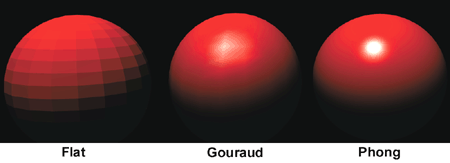
\includegraphics[width=1\linewidth]{images/shading.png}
    \caption{Примеры закрасок}
    \label{shading}
\end{figure}

\subsection{Модели освещения}

\subsubsection{Модель освещения Ламберта}

Модель освещения Ламберта описывает диффузное отражение света, при котором интенсивность отражённого света пропорциональна косинусу угла между направлением света и нормалью к поверхности. Формула имеет вид:

$$
I = I_0 k_a + I_t k_d \cos \theta, \quad 0 \leq \theta \leq \frac{\pi}{2},
$$

где:
\begin{itemize}[label=---]
    \item $I$ — интенсивность отражённого света;
    \item $I_0$ — интенсивность рассеянного света;
    \item $k_a$ — коэффициент диффузного отражения рассеянного света ($0~\leq~k_a~\leq~1$);
    \item $I_t$ — интенсивность точечного источника света;
    \item $k_d$ — коэффициент диффузного отражения для направленного света ($0 \leq k_d \leq 1$);
    \item $\theta$ — угол между направлением света и нормалью к поверхности.
\end{itemize}

Эта модель предполагает, что поверхность отражает свет равномерно во всех направлениях, а интенсивность освещения зависит от угла падения света.

\begin{figure}[H]
    \centering
    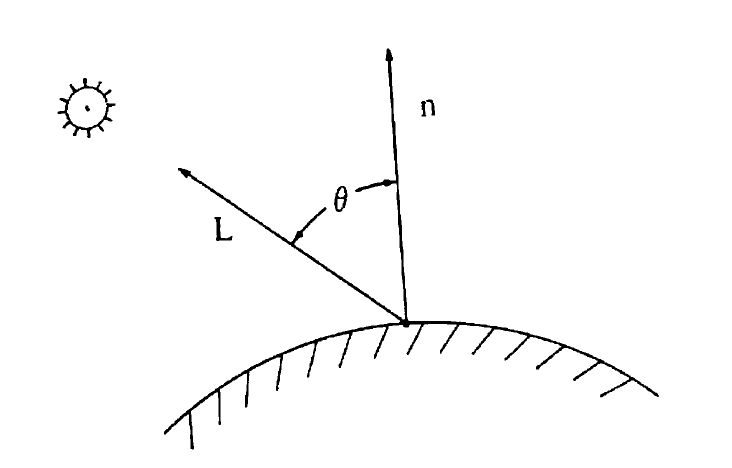
\includegraphics[width=0.8\linewidth]{images/light/lambert.png}
    \caption{Схема модели освещения Ламберта}
    \label{fig:lambert}
\end{figure}

\textbf{Преимущества:} Такой подход хорошо подходит для диффузных и матовых поверхностей.

\textbf{Недостатки:} не учитывает бликов и подходит только для равномерно освещённых объектов.

\subsubsection{Модель освещения Фонга}

Модель освещения Фонга расширяет модель Ламберта за счёт добавления зеркального отражения, описывающего поведение света на глянцевых поверхностях. Она состоит из трёх компонентов освещения: фонового, диффузного и зеркального. Формула имеет вид:

$$
I = I_0 k_a + \frac{I_t k_d \cos \theta}{d + K} + I_t k_s \cos^n \alpha,
$$

где:
\begin{itemize}[label=---]
    \item $I$ — общая интенсивность света;
    \item $I_0$ — интенсивность фонового рассеянного света;
    \item $k_a$ — коэффициент фонового освещения;
    \item $I_t$ — интенсивность направленного источника света;
    \item $k_d$ — коэффициент диффузного отражения;
    \item $\cos \theta$ — косинус угла между нормалью к поверхности и направлением света;
    \item $d$ — расстояние от источника света до объекта;
    \item $K$ — произвольная постоянная для уменьшения интенсивности с расстоянием;
    \item $k_s$ — коэффициент зеркального отражения;
    \item $\cos \alpha$ — косинус угла между направлением отражённого света и направлением наблюдателя;
    \item $n$ — степень блеска, управляющая шириной блика (чем больше $n$, тем уже блик).
\end{itemize}

Модель Фонга описывает, как свет распределяется на поверхности: диффузный компонент учитывает матовое отражение, а зеркальный — глянцевый блик, зависящий от угла обзора и гладкости поверхности.

\begin{figure}[H]
    \centering
    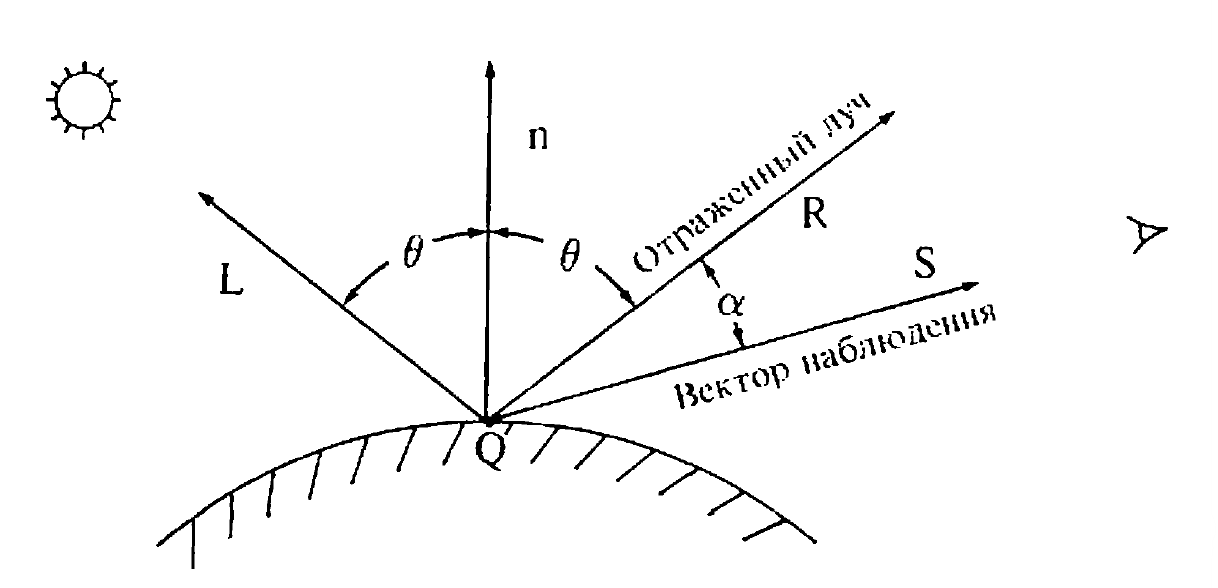
\includegraphics[width=0.8\linewidth]{images/light/phong.png}
    \caption{Схема модели освещения Фонга}
    \label{fig:lambert}
\end{figure}


\textbf{Преимущества:} реалистичное освещение, подходящее для сложных сцен и объектов.

\textbf{Недостатки:} сложность вычислений.

\subsection{Выбор методов}

Для визуализации тел вращения оптимальным выбором являются Z-буфер, модель освещения Ламберта и закраска по Фонгу. Такое сочетание методов обеспечит высокое качество визуализации с учётом света, тени и цвета, а также на выходе получится реалистичное изображение.

\paragraph*{ВЫВОД} ${}$ \\

В данном разделе проанализированы доступные алгоритмы, предназначенные для генерации кривой Безье, генерации и визуализации тел вращения. Также обоснован выбор предложенных методов и описаны ограничения, в которых будет функционировать создаваемое программное обеспечение.
